\documentclass[preview]{standalone}

\usepackage{amsmath}
\usepackage{amssymb}
\usepackage{stellar}
\usepackage{definitions}
\usepackage{enumitem}
\usepackage{tikz}

\begin{document}

\id{integrals-on-curves-exercises}
\genpage

\section{Exercises}

\begin{snippetexercise}{integrals-on-curves-ex1}{}
    \textbf{1.} Let \( \Gamma \) be the curve defined by:
    \[
        \Gamma : \begin{cases} 
        x + y = 1 \\ 
        z = y^2 - 2x^2 \\ 
        x \ge 0, \, y \ge 0, \, z \ge 0. 
        \end{cases}
    \]

    \begin{enumerate}[label=\roman*)]
        \item Write a parametrization of \( \Gamma \);
        \item Let \( f : \realnumbers^3 \to \realnumbers \) be defined by
        \[
            f(x,y,z) = x^2 + z - 3.
        \]
        Calculate \( \displaystyle \int_{\Gamma} f \, ds \).
    \end{enumerate}
\end{snippetexercise}

\begin{snippetsolution}{integrals-on-curves-ex1-sol}{}
    \begin{enumerate}
        \item We can choose \( x = t \) as the parameter. From the first equation, we have \( y = 1 - t \).
            Substituting these into the second equation yields:
            \[
                z = (1-t)^2 - 2t^2 = 1 - 2t + t^2 - 2t^2 = 1 - 2t - t^2.
            \]
            To determine the domain of the parameter \( t \), we impose the given inequalities:
            \begin{itemize}
                \item \( x \ge 0 \implies t \ge 0 \).
                \item \( y \ge 0 \implies 1 - t \ge 0 \implies t \le 1 \).
                \item \( z \ge 0 \implies 1 - 2t - t^2 \ge 0 \implies t^2 + 2t - 1 \le 0 \).
            \end{itemize}
            The roots of \( t^2 + 2t - 1 = 0 \) are \( t = \frac{-2 \pm \sqrt{4 - 4(-1)}}{2} = -1 \pm \sqrt{2} \). Since the leading coefficient is positive, the inequality \( t^2 + 2t - 1 \le 0 \) holds between the roots:
            \[
                -1 - \sqrt{2} \le t \le -1 + \sqrt{2}.
            \]
            Intersecting all conditions (\( 0 \le t \le 1 \) and \( t \le \sqrt{2}-1 \)), the domain is \( t \in [0, \sqrt{2}-1] \).
            
            Thus, the parametrization is:
            \[
                r(t) = \left( t, \, 1-t, \, 1-2t-t^2 \right), \quad t \in [0, \sqrt{2}-1].
            \]
        \item The line integral is computed as \( \int_{\Gamma} f \, ds = \int_a^b f(r(t)) \| r'(t) \| \, dt \).
            First, evaluate \( f \) along the curve:
            \[
                f(r(t)) = x(t)^2 + z(t) - 3 = t^2 + (1 - 2t - t^2) - 3 = -2t - 2 = -2(t+1).
            \]
            Next, compute the magnitude of the tangent vector \( r'(t) \):
            \[
                r'(t) = \frac{d}{dt} \left( t, \, 1-t, \, 1-2t-t^2 \right) = (1, \, -1, \, -2 - 2t).
            \]
            \[
                \| r'(t) \| = \sqrt{1^2 + (-1)^2 + (-2(1+t))^2} = \sqrt{2 + 4(1 + 2t + t^2)} = \sqrt{4t^2 + 8t + 6}.
            \]
            The integral becomes:
            \[
                I = \int_{0}^{\sqrt{2}-1} -2(t+1) \sqrt{4t^2 + 8t + 6} \, dt.
            \]
            Use the substitution \( u = 4t^2 + 8t + 6 \). Then \( du = (8t + 8) \, dt = 8(t+1) \, dt \), which implies \( -2(t+1) \, dt = -\frac{1}{4} \, du \).
            
            Determine the new limits of integration:
            \begin{itemize}
                \item If \( t = 0 \), then \( u = 6 \).
                \item If \( t = \sqrt{2}-1 \):
                \begin{align*}
                    u &= 4(\sqrt{2}-1)^2 + 8(\sqrt{2}-1) + 6 \\
                    &= 4(2 - 2\sqrt{2} + 1) + 8\sqrt{2} - 8 + 6 \\
                    &= 12 - 8\sqrt{2} + 8\sqrt{2} - 2 \\
                    &= 10.
                \end{align*}
            \end{itemize}
            Finally, calculate the integral:
            \[
                I = \int_{6}^{10} -\frac{1}{4} \sqrt{u} \, du = -\frac{1}{4} \left[ \frac{2}{3} u^{3/2} \right]_{6}^{10} = -\frac{1}{6} \left( 10\sqrt{10} - 6\sqrt{6} \right) = \sqrt{6} - \frac{5}{3}\sqrt{10}.
            \]
    \end{enumerate}
\end{snippetsolution}

\begin{snippetexercise}{integrals-on-curves-ex2}{}
    Determine if the following curve is closed, simple, regular:
    \[\gamma(t)=\left(-t^2+2t, t^3-3t^2+2t\right), \quad t \in [-1, 3].\]
\end{snippetexercise}

\begin{snippetsolution}{integrals-on-curves-ex2-sol}{}
    Let \(\gamma(t)=(x(t), y(t))\). To solve the exercise, we analyze the properties of the curve individually.

    \begin{itemize}
        \item \emph{Is the curve closed?}
            A curve is closed if \(\gamma(a)=\gamma(b)\). Here, the interval is \([-1, 3]\).
            Calculations:
            \begin{itemize}
                \item \(\gamma(-1) = \left(-(-1)^2+2(-1), (-1)^3-3(-1)^2+2(-1)\right) = (-1-2, -1-3-2) = (-3, -6)\).
                \item \(\gamma(3) = \left(-3^2+2(3), 3^3-3(3)^2+2(3)\right) = (-9+6, 27-27+6) = (-3, 6)\).
            \end{itemize}
            Since \(\gamma(-1) \neq \gamma(3)\), the curve is \textbf{not closed}.
        \item \emph{Is the curve simple?}
            A curve is simple if it does not intersect itself, meaning \(\gamma(t_1)=\gamma(t_2) \implies t_1=t_2\) (excluding the endpoints for closed curves).
            Let's verify if there are any self-intersections.
            Consider the x-component: \(x(t_1)=x(t_2) \implies -t_1^2+2t_1 = -t_2^2+2t_2\).
            Rearranging terms: \(t_1^2-t_2^2 - 2(t_1-t_2) = 0 \implies (t_1-t_2)(t_1+t_2-2) = 0\).
            For \(t_1 \neq t_2\), we must have \(t_1+t_2=2\), or \(t_2=2-t_1\).

            Now we check if the y-component is equal for these values:
            \(y(t) = t^3-3t^2+2t = t(t^2-3t+2) = t(t-1)(t-2)\).
            The roots of \(y(t)\) are \(t=0, 1, 2\).
            Notice that if we choose \(t_1=0\), then \(t_2=2-0=2\). Both belong to the domain \([-1, 3]\).
            \begin{itemize}
                \item \(\gamma(0) = (0, 0)\)
                \item \(\gamma(2) = (-4+4, 8-12+4) = (0, 0)\)
            \end{itemize}
            Since \(\gamma(0)=\gamma(2)\) with \(0 \neq 2\), the curve has a self-intersection at the origin.
            Therefore, the curve is \textbf{not simple}.
        \item \emph{Is the curve regular?}
            A curve is regular if its tangent vector \(\gamma'(t)\) is never the zero vector in the interior of the domain.
            Compute the derivative:
            \[\gamma'(t) = (x'(t), y'(t)) = (-2t+2, 3t^2-6t+2).\]
            Find where \(x'(t)=0\):
            \(-2t+2=0 \implies t=1\).
            Check the value of \(y'(t)\) at \(t=1\):
            \(y'(1) = 3(1)^2 - 6(1) + 2 = 3 - 6 + 2 = -1 \neq 0\).
            Since the two components never vanish simultaneously, \(\gamma'(t) \neq \vec{0}\) for all \(t \in [-1, 3]\).
            Therefore, the curve is \textbf{regular}.
    \end{itemize}
\end{snippetsolution}

\begin{snippetexercise}{integrals-on-curves-ex3}{}
    Determine if the following curve is closed, simple, regular:
    \[\gamma(t)=\left(\frac{t^2}{1+t^2}, \frac{t^3}{1+t^2}\right), \quad t \in [-5, 5].\]
\end{snippetexercise}

\begin{snippetsolution}{integrals-on-curves-ex3-sol}{}
    Let \(\gamma(t)=(x(t), y(t))\). We analyze the properties of the curve individually.
    \begin{enumerate}
        \item \emph{Is the curve closed?}
        A curve is closed if \(\gamma(a)=\gamma(b)\). Here, the interval is \([-5, 5]\).
        We calculate the values at the endpoints:
        \[x(-5) = \frac{(-5)^2}{1+(-5)^2} = \frac{25}{26}, \quad x(5) = \frac{5^2}{1+5^2} = \frac{25}{26}.\]
        \[y(-5) = \frac{(-5)^3}{1+(-5)^2} = -\frac{125}{26}, \quad y(5) = \frac{5^3}{1+5^2} = \frac{125}{26}.\]
        Since \(y(-5) \neq y(5)\), we have \(\gamma(-5) \neq \gamma(5)\).
        Thus, the curve is \textbf{not closed}.
        \item \emph{Is the curve simple?}
        We check for self-intersections: \(\gamma(t_1)=\gamma(t_2)\) for \(t_1 \neq t_2\).
        From the x-component:
        \[\frac{t_1^2}{1+t_1^2} = \frac{t_2^2}{1+t_2^2} \implies t_1^2(1+t_2^2) = t_2^2(1+t_1^2) \implies t_1^2 = t_2^2.\]
        This implies \(t_1 = t_2\) or \(t_1 = -t_2\). Since we assume \(t_1 \neq t_2\), we must have \(t_1 = -t_2\).
        Now we substitute \(t_1 = -t_2\) into the y-component. Since \(y(t) = \frac{t^3}{1+t^2}\) is an odd function (odd numerator, even denominator):
        \[y(t_1) = y(-t_2) = -y(t_2).\]
        For \(\gamma(t_1)=\gamma(t_2)\), we need \(y(t_1)=y(t_2)\), so \(-y(t_2)=y(t_2) \implies y(t_2)=0\).
        \[\frac{t_2^3}{1+t_2^2} = 0 \implies t_2 = 0.\]
        If \(t_2=0\), then \(t_1=-0=0\), so \(t_1=t_2\), which contradicts the assumption.
        Therefore, there are no distinct points where the curve intersects itself.
        The curve is \textbf{simple}.
        \item \emph{Is the curve regular?}
        We calculate the derivative \(\gamma'(t) = (x'(t), y'(t))\) and check if it is ever the zero vector \(\vec 0\).
        \[x'(t) = \frac{d}{dt}\left(\frac{t^2}{1+t^2}\right) = \frac{2t(1+t^2) - t^2(2t)}{(1+t^2)^2} = \frac{2t}{(1+t^2)^2}.\]
        \[y'(t) = \frac{d}{dt}\left(\frac{t^3}{1+t^2}\right) = \frac{3t^2(1+t^2) - t^3(2t)}{(1+t^2)^2} = \frac{3t^2+t^4}{(1+t^2)^2} = \frac{t^2(3+t^2)}{(1+t^2)^2}.\]
        We check if the derivative vanishes:
        \[x'(t) = 0 \implies 2t = 0 \implies t = 0.\]
        Checking \(y'(t)\) at \(t=0\):
        \[y'(0) = \frac{0(3+0)}{(1+0)^2} = 0.\]
        At \(t=0\), \(\gamma'(0) = (0, 0)\).
        Since the tangent vector vanishes at a point in the domain, the curve is \textbf{not regular}.
    \end{enumerate}
\end{snippetsolution}

\begin{snippetexercise}{integrals-on-curves-ex4}{}
    \todo
\end{snippetexercise}

\begin{snippetsolution}{integrals-on-curves-ex4-sol}{}
    \todo
\end{snippetsolution}

\begin{snippetexercise}{integrals-on-curves-ex5}{Archimedean Spiral}
    Determine if the curve defined by
    \[ \rho = a\theta, \quad \theta \in [0, +\infty), \, a > 0, \]
    is closed, simple, regular. Represent the support of the curve.
\end{snippetexercise}

\begin{snippetsolution}{integrals-on-curves-ex5-sol}{Archimedean Spiral}
    To analyze the curve, we first write its parametrization in Cartesian coordinates using the relations \(x = \rho \cos \theta\) and \(y = \rho \sin \theta\):
    \[ \gamma(\theta) = (a\theta \cos \theta, a\theta \sin \theta), \quad \theta \in [0, +\infty). \]
    \begin{enumerate}
        \item \emph{Is the curve closed?}
        By definition, a curve defined on an interval \([a, b]\) is closed if \(\gamma(a) = \gamma(b)\). In this case, the domain is unbounded \([0, +\infty)\).
        We observe the limit as \(\theta \to +\infty\):
        \[ \|\gamma(\theta)\| = \rho(\theta) = a\theta \xrightarrow{\theta \to +\infty} +\infty. \]
        The curve starts at the origin \(\gamma(0) = (0,0)\) and moves infinitely far away without ever returning to the starting point.
        Therefore, the curve is \textbf{not closed}.

        \item \emph{Is the curve simple?}
        We check if the function \(\gamma\) is injective. Suppose \(\gamma(\theta_1) = \gamma(\theta_2)\). This implies that their distances from the origin must be equal:
        \[ \|\gamma(\theta_1)\| = \|\gamma(\theta_2)\| \implies a\theta_1 = a\theta_2. \]
        Since \(a > 0\), we can divide by \(a\) to get \(\theta_1 = \theta_2\).
        Since distinct parameter values correspond to distinct points in the plane (specifically, points at different distances from the origin), there are no self-intersections.
        Therefore, the curve is \textbf{simple}.

        \item \emph{Is the curve regular?}
        We calculate the derivative vector \(\gamma'(\theta)\) and verify if it vanishes.
        \[ x'(\theta) = \frac{d}{d\theta}(a\theta \cos \theta) = a(\cos \theta - \theta \sin \theta). \]
        \[ y'(\theta) = \frac{d}{d\theta}(a\theta \sin \theta) = a(\sin \theta + \theta \cos \theta). \]
        Now we compute the squared norm of the tangent vector:
        \[ \|\gamma'(\theta)\|^2 = x'(\theta)^2 + y'(\theta)^2 \]
        \[ = a^2 [(\cos \theta - \theta \sin \theta)^2 + (\sin \theta + \theta \cos \theta)^2] \]
        Expanding the squares:
        \[ = a^2 [\cos^2 \theta - 2\theta \cos \theta \sin \theta + \theta^2 \sin^2 \theta + \sin^2 \theta + 2\theta \sin \theta \cos \theta + \theta^2 \cos^2 \theta] \]
        Grouping terms with \(\sin^2 \theta + \cos^2 \theta = 1\):
        \[ = a^2 [(1) + \theta^2(1)] = a^2(1 + \theta^2). \]
        Since \(a > 0\) and \(\theta \ge 0\), the term \(a^2(1+\theta^2)\) is always strictly positive (specifically \(\ge a^2\)).
        Thus, \(\gamma'(\theta) \neq \vec 0\) for all \(\theta\).
        Therefore, the curve is \textbf{regular}.
        \item \emph{Representation of the support}
        The curve starts at the origin and winds counter-clockwise, with the radius increasing linearly with the angle. Below is a representation (assuming \(a=1\)):
        \begin{center}
        \begin{tikzpicture}[scale=0.25]
            \draw[->] (-15,0) -- (15,0) node[right] {$x$};
            \draw[->] (0,-15) -- (0,15) node[above] {$y$};
            % Plotting the Archimedean spiral for theta from 0 to 4pi
            \draw[domain=0:4*pi, samples=200, smooth, thick, blue] plot ({\x*cos(\x r)}, {\x*sin(\x r)});
            \fill (0,0) circle (5pt);
            \node at (1,-1) {\footnotesize $\gamma(0)$};
        \end{tikzpicture}
        \end{center}
    \end{enumerate}
\end{snippetsolution}

\begin{snippetexercise}{integrals-on-curves-ex6}{Logarithmic Spiral}
    Determine if the curve
    \[ \rho = e^\theta, \quad \theta \in \realnumbers, \]
    is closed, simple, regular. Represent the support of the curve and calculate the length of the curve segment for \(\theta \in (-\infty, 0]\).
\end{snippetexercise}

\begin{snippetsolution}{integrals-on-curves-ex6-sol}{Logarithmic Spiral}
    The parametric equations of the curve in Cartesian coordinates are given by:
    \[ \gamma(\theta) = (e^\theta \cos \theta, e^\theta \sin \theta), \quad \theta \in \realnumbers. \]
    \begin{enumerate}
        \item \emph{Is the curve closed?}
        The domain is \(\realnumbers\), which is unbounded. We examine the behavior of the norm:
        \[ \|\gamma(\theta)\| = \rho(\theta) = e^\theta. \]
        As \(\theta \to +\infty\), \(\|\gamma(\theta)\| \to +\infty\). As \(\theta \to -\infty\), \(\|\gamma(\theta)\| \to 0\).
        The curve does not return to a starting point (nor is it periodic).
        Therefore, the curve is \textbf{not closed}.
        \item \emph{Is the curve simple?}
        We check for injectivity: \(\gamma(\theta_1) = \gamma(\theta_2)\).
        The equality of the norms implies:
        \[ \|\gamma(\theta_1)\| = \|\gamma(\theta_2)\| \implies e^{\theta_1} = e^{\theta_2} \implies \theta_1 = \theta_2. \]
        Since the exponential function is strictly monotonic, distinct parameters correspond to distinct points (with different distances from the origin).
        Therefore, the curve is \textbf{simple}.
        \item \emph{Is the curve regular?}
        We calculate the derivative vector \(\gamma'(\theta)\):
        \[ x'(\theta) = e^\theta \cos \theta - e^\theta \sin \theta = e^\theta(\cos \theta - \sin \theta). \]
        \[ y'(\theta) = e^\theta \sin \theta + e^\theta \cos \theta = e^\theta(\sin \theta + \cos \theta). \]
        The squared norm of the tangent vector is:
        \[ \|\gamma'(\theta)\|^2 = x'(\theta)^2 + y'(\theta)^2 = e^{2\theta}[(\cos \theta - \sin \theta)^2 + (\sin \theta + \cos \theta)^2]. \]
        Expanding the terms in the brackets:
        \[ (\cos^2 \theta - 2\sin \theta \cos \theta + \sin^2 \theta) + (\sin^2 \theta + 2\sin \theta \cos \theta + \cos^2 \theta) = 2(\cos^2 \theta + \sin^2 \theta) = 2. \]
        Thus,
        \[ \|\gamma'(\theta)\|^2 = 2e^{2\theta} \implies \|\gamma'(\theta)\| = \sqrt{2}e^\theta. \]
        Since \(e^\theta > 0\) for all \(\theta \in \realnumbers\), \(\|\gamma'(\theta)\| \neq 0\).
        Therefore, the curve is \textbf{regular}.
        \item \emph{Representation of the support}
        The curve spirals outward from the origin as \(\theta\) increases. For \(\theta \to -\infty\), it asymptotically approaches the origin.
        \begin{center}
        \begin{tikzpicture}[scale=0.5]
            \draw[->] (-5,0) -- (5,0) node[right] {$x$};
            \draw[->] (0,-5) -- (0,5) node[above] {$y$};
            % Plotting the logarithmic spiral e^(0.15*theta) to make it visible
            % Using a smaller growth rate for visualization purposes or just mapping e^theta scaled down
            \draw[domain=-10:2.5, samples=300, smooth, thick, red] plot ({0.5*exp(\x)*cos(\x r)}, {0.5*exp(\x)*sin(\x r)});
        \end{tikzpicture}
        \end{center}
        \item \emph{Calculation of the length}
        We need to calculate the length of the curve for \(\theta \in (-\infty, 0]\). This is an improper integral:
        \[ L = \int_{-\infty}^{0} \|\gamma'(\theta)\| \, d\theta = \int_{-\infty}^{0} \sqrt{2}e^\theta \, d\theta. \]
        \[ L = \sqrt{2} \lim_{b \to -\infty} \int_{b}^{0} e^\theta \, d\theta = \sqrt{2} \lim_{b \to -\infty} \left[ e^\theta \right]_b^0. \]
        \[ L = \sqrt{2} (e^0 - \lim_{b \to -\infty} e^b) = \sqrt{2}(1 - 0) = \sqrt{2}. \]
    \end{enumerate}
\end{snippetsolution}

\begin{snippetexercise}{integrals-on-curves-ex7}{Conics in polar coordinates}
    Let \(\varepsilon \ge 0\) and \(\ell > 0\) be constants. Prove that the following curve, described in polar coordinates by
    \[ \rho = \frac{\ell}{1 + \varepsilon \cos \theta} \]
    and defined for values of \(\theta\) that make \(\rho\) positive, is a conic. More precisely, prove that it is an ellipse if \(\varepsilon < 1\), a parabola if \(\varepsilon = 1\), and a hyperbola if \(\varepsilon > 1\).
\end{snippetexercise}

\begin{snippetsolution}{integrals-on-curves-ex7-sol}{}
    To classify the curve, we convert the equation from polar coordinates \((\rho, \theta)\) to Cartesian coordinates \((x, y)\).
    We use the relations:
    \[ x = \rho \cos \theta, \quad y = \rho \sin \theta, \quad \rho = \sqrt{x^2+y^2}. \]
    Starting from the given equation:
    \[ \rho = \frac{\ell}{1 + \varepsilon \cos \theta} \]
    Multiply both sides by the denominator:
    \[ \rho(1 + \varepsilon \cos \theta) = \ell \implies \rho + \varepsilon (\rho \cos \theta) = \ell. \]
    Substitute \(x = \rho \cos \theta\):
    \[ \rho + \varepsilon x = \ell \implies \rho = \ell - \varepsilon x. \]
    Squaring both sides (noting that \(\rho^2 = x^2 + y^2\)):
    \[ x^2 + y^2 = (\ell - \varepsilon x)^2. \]
    Expand the right side:
    \[ x^2 + y^2 = \ell^2 - 2\ell\varepsilon x + \varepsilon^2 x^2. \]
    Group the terms involving \(x\) and \(y\):
    \[ x^2(1 - \varepsilon^2) + 2\ell\varepsilon x + y^2 = \ell^2. \]
    This is the general equation of a conic section. We now analyze the cases based on the value of \(\varepsilon\) (eccentricity).
    \begin{enumerate}
        \item \emph{Case \(\varepsilon = 1\) (Parabola)}
        If \(\varepsilon = 1\), the term \(x^2(1 - \varepsilon^2)\) vanishes. The equation becomes:
        \[ 0 \cdot x^2 + 2\ell(1) x + y^2 = \ell^2 \implies y^2 = \ell^2 - 2\ell x. \]
        Rearranging:
        \[ y^2 = -2\ell \left(x - \frac{\ell}{2}\right). \]
        This is the equation of a \textbf{parabola} with a horizontal axis of symmetry.
        \item \emph{Case \(\varepsilon < 1\) (Ellipse)}
        If \(\varepsilon < 1\), then \(1 - \varepsilon^2 > 0\). The coefficients of \(x^2\) and \(y^2\) are both positive.
        We can complete the square for \(x\). rewrite the equation as:
        \[ (1-\varepsilon^2)\left(x^2 + \frac{2\ell\varepsilon}{1-\varepsilon^2}x\right) + y^2 = \ell^2. \]
        Adding the completion term inside the parenthesis:
        \[ (1-\varepsilon^2)\left(x + \frac{\ell\varepsilon}{1-\varepsilon^2}\right)^2 - (1-\varepsilon^2)\frac{\ell^2\varepsilon^2}{(1-\varepsilon^2)^2} + y^2 = \ell^2. \]
        Simplifying and moving the constant to the right:
        \[ (1-\varepsilon^2)\left(x + x_0\right)^2 + y^2 = \ell^2 + \frac{\ell^2\varepsilon^2}{1-\varepsilon^2} = \frac{\ell^2(1-\varepsilon^2) + \ell^2\varepsilon^2}{1-\varepsilon^2} = \frac{\ell^2}{1-\varepsilon^2}. \]
        Dividing by the constant on the right (which is positive):
        \[ \frac{(x+x_0)^2}{A^2} + \frac{y^2}{B^2} = 1. \]
        Since both terms are positive and summed, this represents an \textbf{ellipse}.
        \item \emph{Case \(\varepsilon > 1\) (Hyperbola)}
        If \(\varepsilon > 1\), then \(1 - \varepsilon^2 < 0\). Let \(\varepsilon^2 - 1 = k > 0\). The equation becomes:
        \[ -kx^2 + 2\ell\varepsilon x + y^2 = \ell^2. \]
        The coefficients of \(x^2\) and \(y^2\) have opposite signs. Completing the square similarly leads to a standard form:
        \[ -\frac{(x-x_0)^2}{A^2} + \frac{y^2}{B^2} = 1 \quad \text{(or similar depending on signs of constants)}. \]
        Since the quadratic terms have opposite signs, this represents a \textbf{hyperbola}.
    \end{enumerate}
\end{snippetsolution}

\begin{snippetexercise}{integrals-on-curves-ex8}{}
    Parametrize the logarithmic spiral by arc length.
\end{snippetexercise}

\begin{snippetsolution}{integrals-on-curves-ex8-sol}{}
    To parameterize the curve by arc length (also known as natural parametrization), we must first calculate the arc length function \(s(\theta)\) and then invert it to find \(\theta(s)\).
    Recall the logarithmic spiral from Exercise 6:
    \[ \gamma(\theta) = (e^\theta \cos \theta, e^\theta \sin \theta). \]
    We previously calculated the magnitude of the tangent vector:
    \[ \|\gamma'(\theta)\| = \sqrt{2}e^\theta. \]
    \begin{enumerate}
        \item \emph{Calculate the arc length function \(s(\theta)\)}
        We choose the origin (limit as \(\theta \to -\infty\)) as the reference point for the arc length, as the curve spirals out from there.
        \[ s(\theta) = \int_{-\infty}^{\theta} \|\gamma'(u)\| \, du = \int_{-\infty}^{\theta} \sqrt{2}e^u \, du. \]
        \[ s(\theta) = \sqrt{2} \left[ e^u \right]_{-\infty}^{\theta} = \sqrt{2}(e^\theta - 0) = \sqrt{2}e^\theta. \]
        Since \(e^\theta > 0\), we have \(s \in (0, +\infty)\).
        \item \emph{Invert the relation to find \(\theta(s)\)}
        From \(s = \sqrt{2}e^\theta\), we solve for \(\theta\):
        \[ e^\theta = \frac{s}{\sqrt{2}} \implies \theta(s) = \ln\left(\frac{s}{\sqrt{2}}\right). \]
        \item \emph{Substitute \(\theta(s)\) into the original parametrization}
        We substitute \(\theta\) in \(\gamma(\theta)\) with \(\ln(s/\sqrt{2})\).
        Note that \(e^{\theta(s)} = \frac{s}{\sqrt{2}}\).
        \[ \tilde{\gamma}(s) = \left( \frac{s}{\sqrt{2}} \cos\left( \ln\left(\frac{s}{\sqrt{2}}\right) \right), \, \frac{s}{\sqrt{2}} \sin\left( \ln\left(\frac{s}{\sqrt{2}}\right) \right) \right), \quad s > 0. \]
    \end{enumerate}
\end{snippetsolution}

\begin{snippetexercise}{integrals-on-curves-ex9}{}
    Parametrize the graph of the function \( y = \cosh x \) by arc length for \( x \in [0, 5] \).
\end{snippetexercise}

\begin{snippetsolution}{integrals-on-curves-ex9-sol}{}
    The graph of a function \( y = f(x) \) can be naturally parametrized as \( \gamma(t) = (t, f(t)) \). In this case:
    \[ \gamma(t) = (t, \cosh t), \quad t \in [0, 5]. \]
    To find the parametrization by arc length, we follow these steps:
    \begin{enumerate}
        \item \emph{Calculate the speed \(\|\gamma'(t)\|\)}
        Compute the derivative vector:
        \[ \gamma'(t) = (1, \sinh t). \]
        Compute the norm:
        \[ \|\gamma'(t)\| = \sqrt{1^2 + (\sinh t)^2} = \sqrt{1 + \sinh^2 t}. \]
        Using the hyperbolic identity \( \cosh^2 t - \sinh^2 t = 1 \), we have \( 1 + \sinh^2 t = \cosh^2 t \).
        \[ \|\gamma'(t)\| = \sqrt{\cosh^2 t} = \cosh t \quad (\text{since } \cosh t > 0). \]
        \item \emph{Calculate the arc length function \(s(t)\)}
        We measure the arc length starting from \(t = 0\):
        \[ s(t) = \int_{0}^{t} \|\gamma'(u)\| \, du = \int_{0}^{t} \cosh u \, du. \]
        \[ s(t) = [\sinh u]_{0}^{t} = \sinh t - \sinh 0 = \sinh t. \]
        The range for the arc length parameter \(s\) corresponds to \(t \in [0, 5]\):
        \[ s \in [\sinh 0, \sinh 5] = [0, \sinh 5]. \]
        \item \emph{Invert the relation to find \(t(s)\)}
        From \( s = \sinh t \), we solve for \(t\):
        \[ t(s) = \operatorname{arcsinh}(s) = \ln(s + \sqrt{s^2 + 1}). \]
        \item \emph{Substitute \(t(s)\) into the original parametrization}
        We substitute \(t = \operatorname{arcsinh}(s)\) into \(\gamma(t) = (t, \cosh t)\).
        The first component is simply \(\operatorname{arcsinh}(s)\).
        The second component is \(\cosh(\operatorname{arcsinh}(s))\).
        Using the identity \(\cosh x = \sqrt{1 + \sinh^2 x}\), we get:
        \[ \cosh(\operatorname{arcsinh}(s)) = \sqrt{1 + (\sinh(\operatorname{arcsinh}(s)))^2} = \sqrt{1 + s^2}. \]
        Thus, the parametrization by arc length is:
        \[ \tilde{\gamma}(s) = \left( \operatorname{arcsinh}(s), \sqrt{1 + s^2} \right), \quad s \in [0, \sinh 5]. \]
    \end{enumerate}
\end{snippetsolution}

\begin{snippetexercise}{integrals-on-curves-ex10}{Cardioid}
    Determine if the following curve, described in polar coordinates by
    \[ \rho(\theta) = 1 + \cos \theta, \quad \theta \in [-\pi, \pi] \]
    is closed, simple, regular. Represent the support of the curve, determine its length, and parametrize it by arc length.
\end{snippetexercise}

\begin{snippetsolution}{integrals-on-curves-ex10-sol}{Cardioid}
    The curve is given by the polar parametrization:
    \[ \gamma(\theta) = ((1+\cos \theta)\cos \theta, (1+\cos \theta)\sin \theta), \quad \theta \in [-\pi, \pi]. \]
    \begin{enumerate}
        \item \emph{Is the curve closed?}
        We evaluate the polar radius at the endpoints of the interval.
        \[ \rho(-\pi) = 1 + \cos(-\pi) = 1 - 1 = 0. \]
        \[ \rho(\pi) = 1 + \cos(\pi) = 1 - 1 = 0. \]
        Since the radius is zero at both endpoints, the curve starts and ends at the origin (the pole).
        Therefore, \(\gamma(-\pi) = \gamma(\pi) = (0,0)\), and the curve is \textbf{closed}.
        \item \emph{Is the curve simple?}
        Since the curve is closed, we check for injectivity on the interval \((-\pi, \pi)\).
        For \(\theta \in (-\pi, \pi)\), we have \(\cos \theta > -1\), so \(\rho(\theta) = 1 + \cos \theta > 0\).
        In polar coordinates, points with \(\rho > 0\) and distinct angles \(\theta \in (-\pi, \pi)\) correspond to distinct points in the plane.
        The only self-intersection occurs at the endpoints where \(\rho=0\).
        Therefore, the curve is \textbf{simple} (it is a simple closed curve).
        \item \emph{Is the curve regular?}
        We compute the magnitude of the tangent vector in polar coordinates:
        \[ \|\gamma'(\theta)\| = \sqrt{(\rho'(\theta))^2 + (\rho(\theta))^2}. \]
        We have \(\rho'(\theta) = -\sin \theta\).
        \[ \|\gamma'(\theta)\|^2 = (-\sin \theta)^2 + (1 + \cos \theta)^2 = \sin^2 \theta + 1 + 2\cos \theta + \cos^2 \theta. \]
        Using \(\sin^2 \theta + \cos^2 \theta = 1\):
        \[ \|\gamma'(\theta)\|^2 = 2 + 2\cos \theta = 2(1 + \cos \theta). \]
        Using the half-angle identity \(1 + \cos \theta = 2 \cos^2(\frac{\theta}{2})\):
        \[ \|\gamma'(\theta)\|^2 = 4 \cos^2\left(\frac{\theta}{2}\right) \implies \|\gamma'(\theta)\| = 2 \left| \cos\left(\frac{\theta}{2}\right) \right|. \]
        For \(\theta \in [-\pi, \pi]\), \(\frac{\theta}{2} \in [-\frac{\pi}{2}, \frac{\pi}{2}]\), so the cosine is non-negative. Thus, \(\|\gamma'(\theta)\| = 2 \cos(\frac{\theta}{2})\).
        We check for singular points where the derivative vanishes:
        \[ 2 \cos\left(\frac{\theta}{2}\right) = 0 \implies \frac{\theta}{2} = \pm \frac{\pi}{2} \implies \theta = \pm \pi. \]
        The tangent vector is the zero vector at the endpoints (the cusp at the origin).
        Therefore, the curve is \textbf{not regular} on the entire interval (it is regular on \((-\pi, \pi)\)).
        \item \emph{Representation of the support}
        The curve is a cardioid with the cusp at the origin and the main body extending along the positive x-axis.
        \begin{center}
        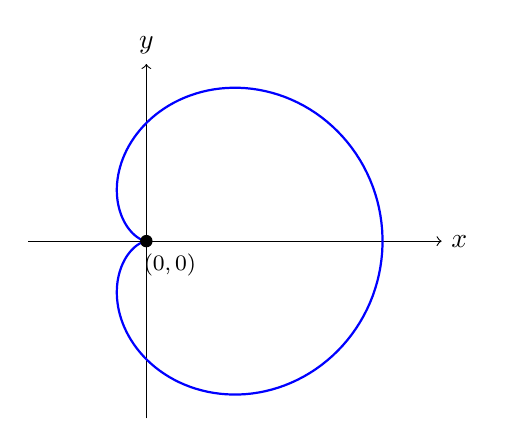
\begin{tikzpicture}[scale=1.5]
            \draw[->] (-1,0) -- (2.5,0) node[right] {$x$};
            \draw[->] (0,-1.5) -- (0,1.5) node[above] {$y$};
            \draw[domain=-180:180, samples=200, thick, blue] plot ({\x}:{1+cos(\x)});
            \fill (0,0) circle (1.5pt);
            \node at (0.2,-0.2) {\footnotesize $(0,0)$};
        \end{tikzpicture}
        \end{center}
        \item \emph{Calculation of the length}
        \[ L = \int_{-\pi}^{\pi} \|\gamma'(\theta)\| \, d\theta = \int_{-\pi}^{\pi} 2 \cos\left(\frac{\theta}{2}\right) \, d\theta. \]
        Let \(u = \frac{\theta}{2}\), then \(du = \frac{1}{2} d\theta \implies d\theta = 2 du\).
        \[ L = \int_{-\pi/2}^{\pi/2} 2 \cos(u) (2 du) = 4 \int_{-\pi/2}^{\pi/2} \cos(u) \, du. \]
        \[ L = 4 [\sin(u)]_{-\pi/2}^{\pi/2} = 4 (1 - (-1)) = 8. \]
        \item \emph{Parametrization by arc length}
        We define the arc length function \(s(\theta)\) starting from \(\theta = -\pi\) (where \(s=0\)):
        \[ s(\theta) = \int_{-\pi}^{\theta} 2 \cos\left(\frac{u}{2}\right) \, du = \left[ 4 \sin\left(\frac{u}{2}\right) \right]_{-\pi}^{\theta}. \]
        \[ s(\theta) = 4 \sin\left(\frac{\theta}{2}\right) - 4 \sin\left(-\frac{\pi}{2}\right) = 4 \sin\left(\frac{\theta}{2}\right) + 4. \]
        Here, \(s\) ranges from \(0\) to \(8\). We invert this relation to find \(\theta(s)\):
        \[ s - 4 = 4 \sin\left(\frac{\theta}{2}\right) \implies \sin\left(\frac{\theta}{2}\right) = \frac{s-4}{4}. \]
        \[ \frac{\theta}{2} = \arcsin\left(\frac{s-4}{4}\right) \implies \theta(s) = 2 \arcsin\left(\frac{s-4}{4}\right). \]
        Substituting this into the original expression for \(\gamma(\theta)\), we obtain the natural parametrization \(\tilde{\gamma}(s) = \gamma(\theta(s))\) for \(s \in [0, 8]\).
        The explicit form is:
        \[ \tilde{\gamma}(s) = \left( \rho(\theta(s)) \cos(\theta(s)), \, \rho(\theta(s)) \sin(\theta(s)) \right), \]
        where \(\theta(s) = 2 \arcsin(\frac{s-4}{4})\) and \(\rho(\theta(s)) = 1 + \cos(2 \arcsin(\frac{s-4}{4})) = 2 - \frac{(s-4)^2}{8}\).
    \end{enumerate}
\end{snippetsolution}

\begin{snippetexercise}{integrals-on-curves-ex11}{Astroid}
    Calculate the length of the curve
    \[ \gamma(t) = (\cos^3 t, \sin^3 t), \quad t \in [0, 2\pi], \]
    and represent it.
\end{snippetexercise}

\begin{snippetsolution}{integrals-on-curves-ex11-sol}{Astroid}
    Let \(\gamma(t) = (x(t), y(t))\).
    \begin{enumerate}
        \item \emph{Representation of the curve}
        The curve is an astroid (a star-shaped hypocycloid with four cusps). The curve is symmetric with respect to both axes and the origin.
        \begin{center}
        \begin{tikzpicture}[scale=2]
            \draw[->] (-1.5,0) -- (1.5,0) node[right] {$x$};
            \draw[->] (0,-1.5) -- (0,1.5) node[above] {$y$};
            \draw[domain=0:360, samples=200, thick, blue] plot ({pow(cos(\x),3)}, {pow(sin(\x),3)});
            \foreach \x/\y in {1/0, 0/1, -1/0, 0/-1}
                \fill (\x,\y) circle (1pt);
            \node at (1.2, -0.2) {1};
            \node at (-0.2, 1.2) {1};
        \end{tikzpicture}
        \end{center}
        \item \emph{Calculation of the derivative}
        We compute the derivatives of the components:
        \[ x'(t) = \frac{d}{dt}(\cos^3 t) = 3\cos^2 t (-\sin t) = -3\cos^2 t \sin t. \]
        \[ y'(t) = \frac{d}{dt}(\sin^3 t) = 3\sin^2 t (\cos t) = 3\sin^2 t \cos t. \]
        \item \emph{Calculation of the norm of the tangent vector}
        \[ \|\gamma'(t)\|^2 = x'(t)^2 + y'(t)^2 \]
        \[ = (-3\cos^2 t \sin t)^2 + (3\sin^2 t \cos t)^2 \]
        \[ = 9\cos^4 t \sin^2 t + 9\sin^4 t \cos^2 t \]
        Factor out \(9\sin^2 t \cos^2 t\):
        \[ = 9\sin^2 t \cos^2 t (\cos^2 t + \sin^2 t) = 9\sin^2 t \cos^2 t. \]
        Taking the square root:
        \[ \|\gamma'(t)\| = \sqrt{9\sin^2 t \cos^2 t} = 3 |\sin t \cos t|. \]
        Using the identity \(\sin(2t) = 2\sin t \cos t\), we can also write this as:
        \[ \|\gamma'(t)\| = \frac{3}{2} |\sin(2t)|. \]
        \item \emph{Calculation of the length}
        The length is given by \(L = \int_0^{2\pi} \|\gamma'(t)\| \, dt\).
        Due to the symmetry of the astroid, the total length is 4 times the length of the curve in the first quadrant (\(t \in [0, \pi/2]\)).
        In the first quadrant, \(\sin t \ge 0\) and \(\cos t \ge 0\), so \(|\sin t \cos t| = \sin t \cos t\).
        \[ L = 4 \int_{0}^{\pi/2} 3 \sin t \cos t \, dt = 12 \int_{0}^{\pi/2} \sin t \cos t \, dt. \]
        We can solve this integral by substitution. Let \(u = \sin t\), then \(du = \cos t \, dt\).
        Limits: \(t=0 \to u=0\), \(t=\pi/2 \to u=1\).
        \[ L = 12 \int_{0}^{1} u \, du = 12 \left[ \frac{u^2}{2} \right]_{0}^{1} = 12 \left( \frac{1}{2} - 0 \right) = 6. \]
        Alternatively, using \(\sin(2t)\):
        \[ L = \int_0^{2\pi} \frac{3}{2} |\sin(2t)| \, dt = 4 \int_0^{\pi/2} \frac{3}{2} \sin(2t) \, dt = 6 \left[ -\frac{\cos(2t)}{2} \right]_0^{\pi/2} = 6 \left( \frac{1}{2} - (-\frac{1}{2}) \right) = 6. \]
    \end{enumerate}
\end{snippetsolution}

\begin{snippetexercise}{integrals-on-curves-ex12}{Cycloid}
    Calculate the centroid of the cycloid arc
    \[ \gamma(t) = (R(t - \sin t), R(1 - \cos t)), \quad t \in [0, 2\pi], \, R > 0. \]
\end{snippetexercise}

\begin{snippetsolution}{integrals-on-curves-ex12-sol}{Cycloid}
    The coordinates of the centroid \((\bar{x}, \bar{y})\) of a curve \(\gamma\) with length \(L\) are given by:
    \[ \bar{x} = \frac{1}{L} \int_{\gamma} x \, ds, \quad \bar{y} = \frac{1}{L} \int_{\gamma} y \, ds. \]
    \begin{enumerate}
        \item \emph{Calculate the arc length element \(ds\)}
        First, we determine the magnitude of the tangent vector \(\|\gamma'(t)\|\).
        \[ x'(t) = R(1 - \cos t), \quad y'(t) = R\sin t. \]
        \[ \|\gamma'(t)\|^2 = R^2(1 - \cos t)^2 + R^2\sin^2 t = R^2(1 - 2\cos t + \cos^2 t + \sin^2 t). \]
        Since \(\cos^2 t + \sin^2 t = 1\):
        \[ \|\gamma'(t)\|^2 = R^2(2 - 2\cos t) = 2R^2(1 - \cos t). \]
        Using the half-angle identity \(1 - \cos t = 2\sin^2(t/2)\):
        \[ \|\gamma'(t)\|^2 = 4R^2\sin^2(t/2) \implies \|\gamma'(t)\| = 2R |\sin(t/2)|. \]
        Since \(t \in [0, 2\pi]\), we have \(t/2 \in [0, \pi]\), so the sine is non-negative. Thus, \(\|\gamma'(t)\| = 2R \sin(t/2)\).
        The arc length element is \(ds = 2R \sin(t/2) \, dt\).
        \item \emph{Calculate the total length \(L\)}
        \[ L = \int_{0}^{2\pi} 2R \sin(t/2) \, dt = 2R \left[ -2\cos(t/2) \right]_{0}^{2\pi}. \]
        \[ L = -4R (\cos \pi - \cos 0) = -4R (-1 - 1) = 8R. \]
        \item \emph{Calculate \(\bar{x}\)}
        \[ \bar{x} = \frac{1}{L} \int_{0}^{2\pi} x(t) \|\gamma'(t)\| \, dt = \frac{1}{8R} \int_{0}^{2\pi} R(t - \sin t) \cdot 2R \sin(t/2) \, dt. \]
        \[ \bar{x} = \frac{2R^2}{8R} \int_{0}^{2\pi} (t\sin(t/2) - \sin t \sin(t/2)) \, dt = \frac{R}{4} (I_1 - I_2). \]
        Calculating \(I_1 = \int_{0}^{2\pi} t\sin(t/2) \, dt\) by parts:
        \[ I_1 = [-2t\cos(t/2)]_0^{2\pi} + \int_{0}^{2\pi} 2\cos(t/2) \, dt = -4\pi(-1) - 0 + [4\sin(t/2)]_0^{2\pi} = 4\pi. \]
        Calculating \(I_2 = \int_{0}^{2\pi} \sin t \sin(t/2) \, dt\) using \(\sin t = 2\sin(t/2)\cos(t/2)\):
        \[ I_2 = \int_{0}^{2\pi} 2\sin^2(t/2)\cos(t/2) \, dt = \left[ \frac{4}{3}\sin^3(t/2) \right]_0^{2\pi} = 0. \]
        Thus, \(\bar{x} = \frac{R}{4}(4\pi - 0) = \pi R\).
        (Note: This result is expected due to the symmetry of the curve with respect to the line \(x = \pi R\)).
        \item \emph{Calculate \(\bar{y}\)}
        \[ \bar{y} = \frac{1}{L} \int_{0}^{2\pi} y(t) \|\gamma'(t)\| \, dt = \frac{1}{8R} \int_{0}^{2\pi} R(1 - \cos t) \cdot 2R \sin(t/2) \, dt. \]
        Using \(1 - \cos t = 2\sin^2(t/2)\):
        \[ \bar{y} = \frac{2R^2}{8R} \int_{0}^{2\pi} 2\sin^2(t/2) \sin(t/2) \, dt = \frac{R}{2} \int_{0}^{2\pi} \sin^3(t/2) \, dt. \]
        Let \(u = t/2\), then \(dt = 2du\). The limits become \(0\) to \(\pi\).
        \[ \bar{y} = \frac{R}{2} \int_{0}^{\pi} \sin^3 u (2du) = R \int_{0}^{\pi} (1 - \cos^2 u)\sin u \, dt. \]
        Integration yields:
        \[ \bar{y} = R \left[ -\cos u + \frac{\cos^3 u}{3} \right]_0^{\pi} = R \left[ \left(1 - \frac{1}{3}\right) - \left(-1 + \frac{1}{3}\right) \right] = R \left( \frac{2}{3} + \frac{2}{3} \right) = \frac{4}{3}R. \]
        \item \emph{Conclusion}
        The centroid is \( (\bar{x}, \bar{y}) = \left( \pi R, \frac{4}{3}R \right) \).
    \end{enumerate}
\end{snippetsolution}

\begin{snippetexercise}{integrals-on-curves-ex13}{}
    Calculate
    \[ \int_{\Gamma} (x^2 + y^2)^2 \, ds, \]
    where \(\Gamma\) is the curve with polar equation
    \[ \rho = e^{2\theta}, \quad \theta \in (-\infty, 0]. \]
\end{snippetexercise}

\begin{snippetsolution}{integrals-on-curves-ex13-sol}{}
    To calculate the line integral of the scalar field \(f(x,y) = (x^2+y^2)^2\), we express all components in terms of the polar parameter \(\theta\).
    \begin{enumerate}
        \item \emph{Parametrization and Integrand}
        In polar coordinates, the distance from the origin is \(x^2 + y^2 = \rho^2\).
        Given the equation of the curve \(\rho = e^{2\theta}\), the function to be integrated simplifies to:
        \[ f(\gamma(\theta)) = (x^2 + y^2)^2 = (\rho^2)^2 = \rho^4 = (e^{2\theta})^4 = e^{8\theta}. \]
        \item \emph{Arc length element \(ds\)}
        For a curve defined by a polar equation \(\rho = \rho(\theta)\), the arc length element is given by \(ds = \sqrt{\rho(\theta)^2 + \rho'(\theta)^2} \, d\theta\).
        First, calculate the derivative with respect to \(\theta\):
        \[ \rho'(\theta) = \frac{d}{d\theta}(e^{2\theta}) = 2e^{2\theta}. \]
        Now, compute the term inside the square root:
        \[ \rho^2 + (\rho')^2 = (e^{2\theta})^2 + (2e^{2\theta})^2 = e^{4\theta} + 4e^{4\theta} = 5e^{4\theta}. \]
        Thus,
        \[ ds = \sqrt{5e^{4\theta}} \, d\theta = \sqrt{5} e^{2\theta} \, d\theta. \]
        \item \emph{Calculation of the integral}
        We integrate over the given domain \(\theta \in (-\infty, 0]\):
        \[ I = \int_{-\infty}^{0} f(\gamma(\theta)) \, ds = \int_{-\infty}^{0} e^{8\theta} \cdot \sqrt{5} e^{2\theta} \, d\theta. \]
        Combine the exponential terms (\(e^{8\theta} \cdot e^{2\theta} = e^{10\theta}\)):
        \[ I = \sqrt{5} \int_{-\infty}^{0} e^{10\theta} \, d\theta. \]
        Evaluate the improper integral:
        \[ I = \sqrt{5} \lim_{b \to -\infty} \left[ \frac{1}{10} e^{10\theta} \right]_{b}^{0} = \frac{\sqrt{5}}{10} \left( e^0 - \lim_{b \to -\infty} e^{10b} \right). \]
        Since \(e^0 = 1\) and \(\lim_{x \to -\infty} e^x = 0\):
        \[ I = \frac{\sqrt{5}}{10} (1 - 0) = \frac{\sqrt{5}}{10}. \]
    \end{enumerate}
\end{snippetsolution}

\begin{snippetexercise}{integrals-on-curves-ex14}{}
    Calculate \( \displaystyle \int_{\gamma} \mathbf{F} \cdot \mathbf{T} \, ds \), where
    \[ \gamma(t) = (t - \sin t, 1 - \cos t, t^2), \quad t \in \left[0, \frac{\pi}{2}\right] \]
    and
    \[ \mathbf{F}(x, y, z) = (\sqrt{z}, x, y). \]
\end{snippetexercise}

\begin{snippetsolution}{integrals-on-curves-ex14-sol}{}
    The integral \( \int_{\gamma} \mathbf{F} \cdot \mathbf{T} \, ds \) is equivalent to the line integral of the second kind \( \int_{\gamma} \mathbf{F} \cdot d\mathbf{r} \).
    The calculation is performed using the formula:
    \[ I = \int_{a}^{b} \mathbf{F}(\gamma(t)) \cdot \gamma'(t) \, dt. \]
    \begin{enumerate}
        \item \emph{Calculate the tangent vector \(\gamma'(t)\)}
        \[ x'(t) = \frac{d}{dt}(t - \sin t) = 1 - \cos t. \]
        \[ y'(t) = \frac{d}{dt}(1 - \cos t) = \sin t. \]
        \[ z'(t) = \frac{d}{dt}(t^2) = 2t. \]
        Thus, \(\gamma'(t) = (1 - \cos t, \sin t, 2t)\).
        \item \emph{Evaluate the vector field \(\mathbf{F}\) on the curve}
        Substitute \(x(t), y(t), z(t)\) into \(\mathbf{F}(x,y,z) = (\sqrt{z}, x, y)\):
        \begin{itemize}
            \item First component: \(\sqrt{z(t)} = \sqrt{t^2} = |t|\). Since \(t \in [0, \pi/2]\), \(\sqrt{t^2} = t\).
            \item Second component: \(x(t) = t - \sin t\).
            \item Third component: \(y(t) = 1 - \cos t\).
        \end{itemize}
        So, \(\mathbf{F}(\gamma(t)) = (t, t - \sin t, 1 - \cos t)\).
        \item \emph{Compute the dot product}
        \[ \mathbf{F}(\gamma(t)) \cdot \gamma'(t) = t(1 - \cos t) + (t - \sin t)(\sin t) + (1 - \cos t)(2t). \]
        Expanding the terms:
        \[ = t - t\cos t + t\sin t - \sin^2 t + 2t - 2t\cos t. \]
        Grouping like terms:
        \[ = 3t - 3t\cos t + t\sin t - \sin^2 t. \]
        \item \emph{Calculate the integral}
        \[ I = \int_{0}^{\pi/2} (3t - 3t\cos t + t\sin t - \sin^2 t) \, dt. \]
        We integrate term by term:
        \begin{itemize}
            \item \(\int 3t \, dt = \frac{3}{2}t^2\).
            \item \(\int -3t\cos t \, dt\): Using integration by parts (\(u=t, dv=\cos t dt\)),
            \[ -3(t\sin t - \int \sin t \, dt) = -3(t\sin t + \cos t). \]
            \item \(\int t\sin t \, dt\): Using integration by parts (\(u=t, dv=\sin t dt\)),
            \[ -t\cos t - \int (-\cos t) \, dt = -t\cos t + \sin t. \]
            \item \(\int -\sin^2 t \, dt = \int -\frac{1 - \cos(2t)}{2} \, dt = -\frac{1}{2}t + \frac{1}{4}\sin(2t)\).
        \end{itemize}
        Combining the primitives:
        \[ I = \left[ \frac{3}{2}t^2 - 3t\sin t - 3\cos t - t\cos t + \sin t - \frac{1}{2}t + \frac{1}{4}\sin(2t) \right]_{0}^{\pi/2}. \]
        Simplifying the expression inside the brackets:
        \[ G(t) = \frac{3}{2}t^2 - \frac{1}{2}t - 3t\sin t - (3+t)\cos t + \sin t + \frac{1}{4}\sin(2t). \]
        Evaluate at \(t = \frac{\pi}{2}\):
        \[ G\left(\frac{\pi}{2}\right) = \frac{3}{2}\frac{\pi^2}{4} - \frac{\pi}{4} - 3\frac{\pi}{2}(1) - 0 + 1 + 0 = \frac{3\pi^2}{8} - \frac{\pi}{4} - \frac{6\pi}{4} + 1 = \frac{3\pi^2}{8} - \frac{7\pi}{4} + 1. \]
        Evaluate at \(t = 0\):
        \[ G(0) = 0 - 0 - 0 - 3(1) + 0 + 0 = -3. \]
        Finally:
        \[ I = G\left(\frac{\pi}{2}\right) - G(0) = \left( \frac{3\pi^2}{8} - \frac{7\pi}{4} + 1 \right) - (-3) = \frac{3\pi^2}{8} - \frac{7\pi}{4} + 4. \]
    \end{enumerate}
\end{snippetsolution}

\begin{snippetexercise}{integrals-on-curves-ex15}{}
    Determine if the vector field
    \[ \mathbf{F}(x, y, z) = \left(x^2, y, z^3\right) \]
    is conservative in \(\realnumbers^3\) and determine a potential, if it exists.
\end{snippetexercise}

\begin{snippetsolution}{integrals-on-curves-ex15-sol}{}
    To determine if the field is conservative, we must verify that its curl is zero (irrotational) and that the domain is simply connected.
    The domain is \(\realnumbers^3\), which is simply connected.
    \begin{enumerate}
        \item \emph{Check the curl \(\gradient \times \mathbf{F}\)}
        Let \(\mathbf{F} = (F_1, F_2, F_3) = (x^2, y, z^3)\).
        \[
        \gradient \times \mathbf{F} = \det \begin{pmatrix} \mathbf{i} & \mathbf{j} & \mathbf{k} \\ \partial_x & \partial_y & \partial_z \\ x^2 & y & z^3 \end{pmatrix}
        \]
        \[
        = \left( \frac{\partial(z^3)}{\partial y} - \frac{\partial(y)}{\partial z}, \quad \frac{\partial(x^2)}{\partial z} - \frac{\partial(z^3)}{\partial x}, \quad \frac{\partial(y)}{\partial x} - \frac{\partial(x^2)}{\partial y} \right).
        \]
        Since the components \(F_1, F_2, F_3\) depend only on \(x, y, z\) respectively, the mixed derivatives are all zero:
        \[
        = (0 - 0, \, 0 - 0, \, 0 - 0) = \mathbf{0}.
        \]
        Since \(\gradient \times \mathbf{F} = \mathbf{0}\) on a simply connected domain, \(\mathbf{F}\) is \textbf{conservative}.
        \item \emph{Calculation of the potential \(\phi\)}
        We look for a function \(\phi(x,y,z)\) such that \(\gradient \phi = \mathbf{F}\).
        \[
        \begin{cases}
            \partial_x \phi = x^2 \\
            \partial_y \phi = y \\
            \partial_z \phi = z^3
        \end{cases}
        \]
        Integrating the first equation with respect to \(x\):
        \[ \phi(x,y,z) = \int x^2 \, dx = \frac{x^3}{3} + C_1(y,z). \]
        Differentiating with respect to \(y\) and equating to \(F_2\):
        \[ \partial_y \left( \frac{x^3}{3} + C_1(y,z) \right) = \partial_y C_1(y,z) = y. \]
        Integrating with respect to \(y\):
        \[ C_1(y,z) = \frac{y^2}{2} + C_2(z). \]
        Updating \(\phi\):
        \[ \phi(x,y,z) = \frac{x^3}{3} + \frac{y^2}{2} + C_2(z). \]
        Differentiating with respect to \(z\) and equating to \(F_3\):
        \[ \partial_z \left( \frac{x^3}{3} + \frac{y^2}{2} + C_2(z) \right) = C_2'(z) = z^3. \]
        Integrating with respect to \(z\):
        \[ C_2(z) = \frac{z^4}{4} + C. \]
        
        Thus, the potential is:
        \[ \phi(x,y,z) = \frac{x^3}{3} + \frac{y^2}{2} + \frac{z^4}{4} + C, \quad C \in \realnumbers. \]
    \end{enumerate}
\end{snippetsolution}

\begin{snippetexercise}{integrals-on-curves-ex16}{}
    Consider the central force field
    \[ \mathbf{F}(x, y, z) = \frac{g'(r)}{r}(x, y, z), \]
    where \( r(x, y, z) = \sqrt{x^2 + y^2 + z^2} \) and \( g \) is a function of class \( C^2(\realnumbers) \).
    Prove that \( \mathbf{F} \) is conservative on \( \realnumbers^3 \setminus \{(0, 0, 0)\} \) and calculate a potential.
\end{snippetexercise}

\begin{snippetsolution}{integrals-on-curves-ex16-sol}{}
    A vector field \( \mathbf{F} \) is conservative in a domain \( D \) if there exists a scalar function \( \phi \) (called potential) such that \( \mathbf{F} = \gradient \phi \) in \( D \).
    We are given the field:
    \[ \mathbf{F}(\mathbf{r}) = \frac{g'(r)}{r} \mathbf{r}, \quad \text{where } \mathbf{r} = (x, y, z) \text{ and } r = \|\mathbf{r}\|. \]
    \begin{enumerate}
        \item \emph{Hypothesis for the potential}
        Since the field is central and depends on the radial distance \( r \), it is natural to look for a potential that also depends only on \( r \). Let's test the function:
        \[ \phi(x, y, z) = g(r). \]
        \item \emph{Verification}
        We compute the gradient of \( \phi \). By the chain rule:
        \[ \gradient \phi = \gradient (g(r)) = g'(r) \gradient r. \]
        Now we calculate \( \gradient r \):
        \[ \frac{\partial r}{\partial x} = \frac{\partial}{\partial x} \sqrt{x^2 + y^2 + z^2} = \frac{1}{2\sqrt{x^2 + y^2 + z^2}} (2x) = \frac{x}{r}. \]
        By symmetry, \( \frac{\partial r}{\partial y} = \frac{y}{r} \) and \( \frac{\partial r}{\partial z} = \frac{z}{r} \).
        Thus,
        \[ \gradient r = \left( \frac{x}{r}, \frac{y}{r}, \frac{z}{r} \right) = \frac{\mathbf{r}}{r}. \]
        Substituting this back into the expression for the gradient of \( \phi \):
        \[ \gradient \phi = g'(r) \frac{\mathbf{r}}{r} = \frac{g'(r)}{r} (x, y, z). \]
        \item \emph{Conclusion}
        We observe that the calculated gradient \( \gradient \phi \) is exactly equal to the given vector field \( \mathbf{F} \):
        \[ \gradient g(r) = \mathbf{F}(x, y, z). \]
        Since we have found a scalar potential \( \phi = g(r) \) defined on \( \realnumbers^3 \setminus \{(0, 0, 0)\} \), the vector field \( \mathbf{F} \) is \textbf{conservative}.
        
        The potential is:
        \[ U(x,y,z) = g\left(\sqrt{x^2 + y^2 + z^2}\right) + C. \]
    \end{enumerate}
\end{snippetsolution}

\begin{snippetexercise}{integrals-on-curves-ex17}{}
    Calculate
    \[ \int_{\gamma} \frac{\cos\sqrt{x^2+y^2+z^2}}{\sqrt{x^2+y^2+z^2}} (x \, dx + y \, dy + z \, dz), \]
    where
    \[ \gamma(t) = \left(e^t \sin t, e^t(\cos t + 1), t\right), \quad t \in [0, \pi]. \]
\end{snippetexercise}

\begin{snippetsolution}{integrals-on-curves-ex17-sol}{}
    Let \( r = \sqrt{x^2+y^2+z^2} \). The integral can be interpreted as the line integral \( \int_\gamma \mathbf{F} \cdot d\mathbf{r} \) of the vector field:
    \[ \mathbf{F}(x,y,z) = \left( \frac{x \cos r}{r}, \frac{y \cos r}{r}, \frac{z \cos r}{r} \right) = \frac{\cos r}{r} \mathbf{r}. \]
    \begin{enumerate}
        \item \emph{Identify the potential}
        The vector field is a central field of the form \( f(r)\mathbf{r} \). From Exercise 16, we know that such fields are conservative if we can find a potential \( \phi(r) \).
        Recall that \( \gradient \phi(r) = \phi'(r) \frac{\mathbf{r}}{r} \).
        Comparing this to our field \( \mathbf{F} = \frac{\cos r}{r} \mathbf{r} \), we need:
        \[ \phi'(r) = \cos r. \]
        Integrating with respect to \( r \), we find:
        \[ \phi(r) = \sin r. \]
        Thus, the scalar potential is \( \phi(x,y,z) = \sin\left(\sqrt{x^2+y^2+z^2}\right) \).
        \item \emph{Evaluate the endpoints of the curve}
        Since the field is conservative, the line integral depends only on the values of the potential at the endpoints of the curve \(\gamma\).
        Start point \( A = \gamma(0) \):
        \[ x(0) = e^0 \sin 0 = 0, \quad y(0) = e^0 (\cos 0 + 1) = 2, \quad z(0) = 0. \]
        \[ A = (0, 2, 0) \implies r_A = \sqrt{0^2 + 2^2 + 0^2} = 2. \]
        End point \( B = \gamma(\pi) \):
        \[ x(\pi) = e^\pi \sin \pi = 0, \quad y(\pi) = e^\pi (\cos \pi + 1) = 0, \quad z(\pi) = \pi. \]
        \[ B = (0, 0, \pi) \implies r_B = \sqrt{0^2 + 0^2 + \pi^2} = \pi. \]
        \item \emph{Calculate the integral}
        Using the Fundamental Theorem for Line Integrals:
        \[ I = \int_{\gamma} \gradient \phi \cdot d\mathbf{r} = \phi(B) - \phi(A). \]
        \[ I = \sin(r_B) - \sin(r_A) = \sin(\pi) - \sin(2). \]
        Since \( \sin(\pi) = 0 \):
        \[ I = -\sin 2. \]
    \end{enumerate}
\end{snippetsolution}

\end{document}